\subsection{Radiative Corrections: Overview of Some Famous Radiative Models}

In the context of the Glashow-Weinberg-Salam theory of electroweak interactions it is considered that all the fermions (except the neutrinos) acquire mass through Yukawa couplings with the Higgs boson after spontaneous symmetry breaking. However, in a radiative model this term is forbidden by some symmetry and there is no mass at tree-level, i.e. the zero order mass vanishes, but the mass is generated at loop-level, at \textit{higher order} in the perturbative expansion. In this section we overview some of the famous Radiative collections to neutino masses. 

\subsubsection{Zee-Wolfenstein Model}
One of the most famous radiative model is the so called Zee-Wolfenstein model\cite{zee_wolfstein}. It extends the scalar sector of the SM with two additional scalars: one charged singlet, \(\chi^+\) and one doublet \(\phi_2 = \begin{pmatrix}
    \phi ^+ _2 \\ \phi _2 ^0
\end{pmatrix}\) (the SM Higgs doublet remains). It uses the fact that the  invariant combination of two (different) lepton doublets couples to a  charged scalar singlet, i.e. $(\nu_i l_j - l_i \nu_j) \chi^+$.  By the same  token, two different scalar doublets are also needed, i.e. $(\phi_1^+ \phi_2^0 - \phi_1^0 \phi_2^+) \chi^-$. Moreover \(\phi_2\) is assumed not to couple to leptons. In this model it is not possible to have tree-level neutrino masses from a renormalizeable Lagrangian, but it is possible at one loop level. Such one-loop process is shown in Fig.~\ref{fig:zee_wofl}. Furthermore, the interesting feature of this model is that it suggests a special form for the neutrino mass matrix:

\begin{equation}
\resizebox{0.46\textwidth}{!}{${\cal M}_\mu = \begin{pmatrix}0 & f_{\mu e} (m_\mu^2 - m_e^2) & f_{\tau e} 
(m_\tau^2 - m_e^2) \\  f_{\mu e} (m_\mu^2 - m_e^2) & 0 & f_{\tau \mu} (m_\tau^2 
- m_\mu^2) \\  f_{\tau e} (m_\tau^2 - m_e^2) & f_{\tau \mu} (m_\tau^2 - m_\mu^2) 
& 0 \end{pmatrix}$}
\end{equation}
This model was studied intensively, but it is now ruled out by data\cite{He:2003ih}.

\begin{figure}[!htb]
    \centering
    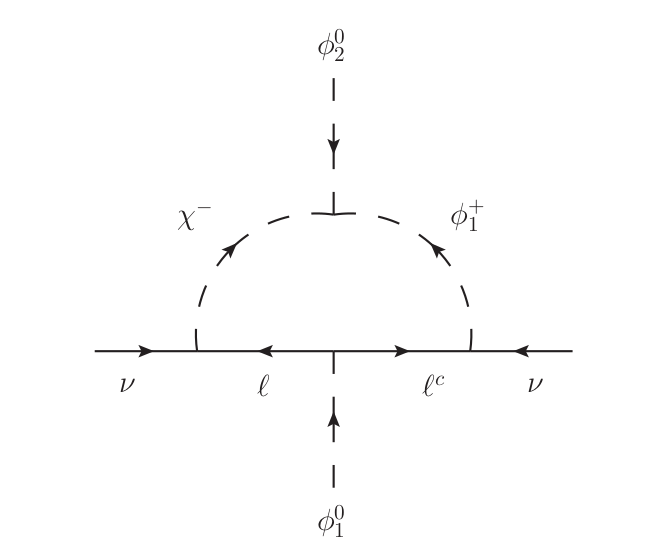
\includegraphics[scale=0.34]{zee_wolf.png}
    \label{fig:zee_wofl}
\caption[]{Zee-Wolfenstein one-loop neutrino mass generation}
\end{figure}

\subsubsection{Zee-Babu Model}


In this model introduced between 1985 and 1987~\cite{Zee:1985id, Babu:1988ki} , the Standard Model is
extended to include two charged singlet Higgs fields: a singly charged $\chi ^+$ and a doubly charged $\xi ^{++}$ , while the right-handed neutrinos are not introduced. The outcome is that the resulting neutrino masses are finite and naturally small, since they arise via two-loop diagrams (see Fig.\ref{fig:zee_babu}). The main prediction of the model is the masslessness of one of the neutrinos but it also predicts that some lepton
number changing decays such as $\mu \to eee$ and $\tau \to \mu \mu \mu$ occur at tree level via $\xi ^{++}$ exchange, which provides a tool for its discovery (as well as it acts as a constraint).
\begin{figure}[!htb]
    \centering
    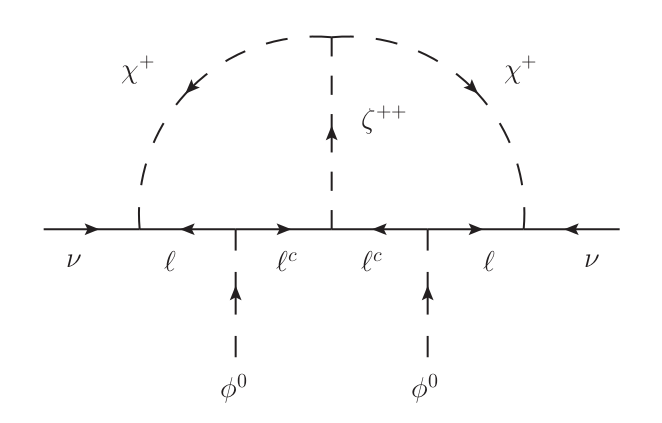
\includegraphics[scale=0.3]{zee_babu.png}
    \label{fig:zee_babu}
\caption[]{Two-loop neutrino mass generation in the Zee-Babu model}
\end{figure}

\subsubsection{Generic 2-W Mechanism in the SM}
As discussed in Sec.~\ref{sub:sm_mass_models}, the minimal model providing mass for the neutrinos is to add just one neutrino singlet $N$. In that simple case, only one linear combination of the flavour eigenstates ($\nu _{e \mu \tau}$) gets a tree-level Majorana mass term while the two others seem to remain massless. However, these zeros are not protected by any symmetry and nothing forces that it remain as such after radiative corrections. And actually as we can see in Fig.~\ref{fig:two_W} there is a two-loop correction generating mass for the other neutrinos. 
\begin{figure}[!htb]
    \centering
    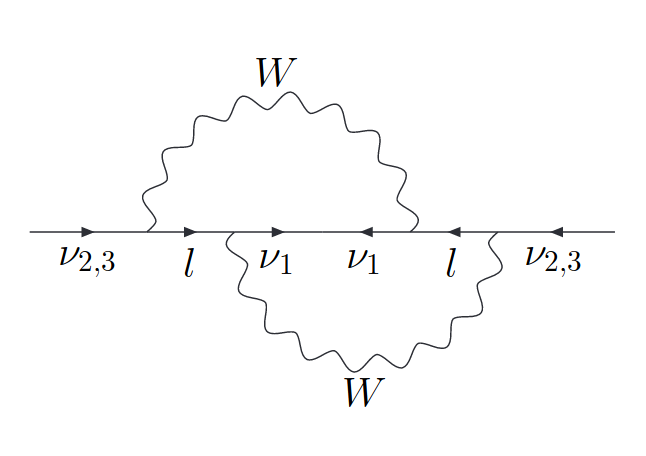
\includegraphics[scale=0.3]{two_W.png}
    \label{fig:two_W}
\caption[]{Two-loop neutrino mass generation in the Zee-Babu model}
\end{figure}

This model introduced in 1988 \cite{babu_ma_phyrev} was formally interesting because although not being totally a radiative model (as one neutrino does have a tree-level mass term) it showed the possibility for the $W$-boson (discovered only five years earlier) to intervene in the generation of neutrino mass only at higher order. However, this two-loop and doubly Glashow-Ilioupoulos-Maiani suppressed mechanism yields completely unsignificant masses for the relevant neutrinos.
%\subsection{Effective Field Theory}
%The effective field theory (EFT) approach is a framework that can be used to describe the generation of neutrino masses. In this approach, the heavy particles that mediate the neutrino masses are integrated out, leaving an effective theory that describes the interactions of the lighter particles that remain. This approach can be used to study the physics at energies below the masses of the heavy particles and provides a simpler and more efficient way of calculating the effects of these heavy particles.

%The EFT approach to neutrino mass generation involves adding new terms to the Standard Model Lagrangian that describe the interactions between the light neutrinos and the heavy particles that mediate their masses. These heavy particles are often assumed to be very massive and not directly observable, but they can still have an impact on the low-energy physics of neutrinos.

%The effective Lagrangian for neutrino mass generation can be written as:

%\begin{equation}
%\mathcal{L}{\text{eff}} = \frac{f{ij}}{\Lambda} \left( \bar{\nu}{L_i} \tilde{\phi} \right) \left( \tilde{\phi}^T \bar{\nu}{L_j}^c \right) + \text{h.c.}
%\end{equation}

%where $\nu_{L_i}$ and $\nu_{L_j}$ are the left-handed neutrino fields of different flavors, $\phi$ is the Higgs field, $\tilde{\phi} = i\sigma_2 \phi^*$, $\sigma_2$ is the second Pauli matrix, and $f_{ij}$ is a complex matrix of coupling constants that depend on the specific model. $\Lambda$ is the energy scale associated with the heavy particles that mediate the neutrino masses. This energy scale is typically much higher than the electroweak scale, which is the scale associated with the Higgs field.

%Using this effective Lagrangian, we can calculate the neutrino masses by diagonalizing the $f_{ij}$ matrix. The mass matrix for the light neutrinos is given by:

%\begin{equation}
%m_{ij} = \frac{v^2}{\Lambda} f_{ij},
%\end{equation}

%where $v$ is the vacuum expectation value of the Higgs field.

%The diagonalization of the $f_{ij}$ matrix can be performed using the Pontecorvo-Maki-Nakagawa-Sakata (PMNS) matrix, which describes the mixing between the different neutrino flavors.